\documentclass{standalone}
\usepackage{unicode-math}
\usepackage{amsmath}
\usepackage{tikz}
\usepackage{fontspec}
\setmainfont{DejaVu Sans}

\usetikzlibrary{automata,arrows,positioning,calc}

\begin{document}

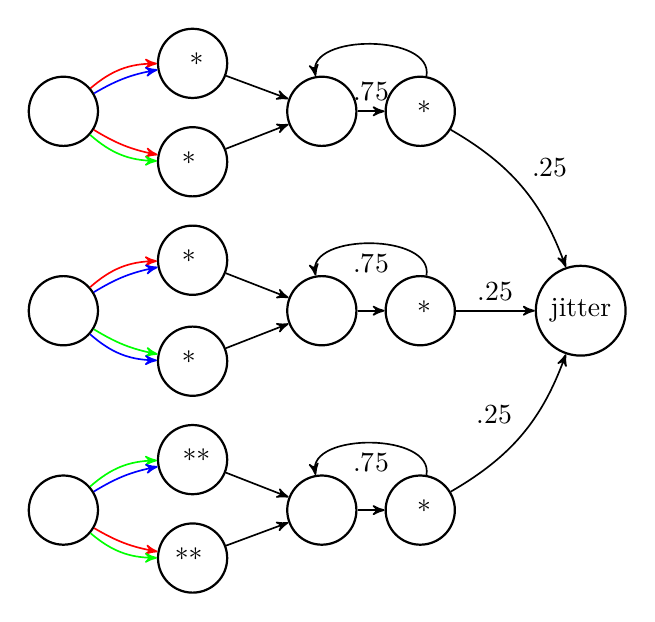
\begin{tikzpicture}[->, >=stealth', auto, semithick, node distance=1.25cm]
    \tikzstyle{every state}=[fill=white,draw=black,thick,text=black,scale=1]

    \node[state] (☺){☺};        %happy
    \node[state] (😏*)[above right=0cm and 1cm of ☺]                     {*😏}; %happy congruent
    \node[state] (*😏)[below right=0cm and 1cm of ☺]                     {*😏}; %happy incongruent
    \node[state] (☺2)[below right=0cm and 1cm of 😏*] {☺};        %happy2
    \node[state] (☺*)[right of=☺2] {☺*}; %happy null

    \node[state] (*😒)[above of=😏*]                     {*😒}; %neutral incongruent
    \node[state] (😐)[above left =0cm and 1cm of *😒]             {😐}; %neutral
    \node[state] (😒*)[above of=*😒]                     {😒*}; %neutral congruent
    \node[state] (😐2)[above right =0cm and 1cm of *😒]             {😐}; %neutral
    \node[state] (😐*)[right of=😐2]                     {😐*}; %neutral null

    \node[state] (😒**)[below of=*😏]   {😒**}; %sad congruent
    \node[state] (☹)[below left=0cm and 1cm of 😒**] {☹};         %sad
    \node[state] (**😒)[below of=😒**] {**😒}; %sad incongruent
    \node[state] (☹2)[below right=0cm and 1cm of 😒**] {☹};         %sad
    \node[state] (☹*)[right of=☹2]                     {☹*}; %sad null

    % fixation point
    \node[state] (jitter)[right=1cm of ☺*] {jitter};  % both's sum = 1800 ms. {{500,1300},{800,1000}}

    % edges
    \path (😐) edge[bend left=20,red] (😒*);
    \path (😐) edge[bend left=10,blue] (😒*);
    \path (😐) edge[bend right=10,red] (*😒);
    \path (😐) edge[bend right=20,green] (*😒);

    \path(☺) edge[bend left=20,red] (😏*);
    \path(☺) edge[bend left=10,blue] (😏*);
    \path(☺) edge[bend right=10,green] (*😏);
    \path(☺) edge[bend right=20,blue] (*😏);

    \path(☹) edge[bend left=20,green] (😒**);
    \path(☹) edge[bend left=10,blue] (😒**);
    \path(☹) edge[bend right=10,red] (**😒);
    \path(☹) edge[bend right=20,green] (**😒);

    % 2nd-to-3rd column edges
    \path(😒*) edge (😐2);
    \path(*😒) edge (😐2);
    \path(😐2) edge node{$.75$} (😐*);
    \path(😐*) edge[bend right=100] (😐2);
    \path(😐*) edge[bend left=20] node{$.25$}  (jitter);

    \path(😏*) edge (☺2);
    \path(*😏) edge (☺2);
    \path(☺2) edge (☺*);
    \path(☺*) edge[bend right=100] node{$.75$} (☺2);
    \path(☺*) edge node{$.25$} (jitter);

    \path(😒**) edge (☹2);
    \path(**😒) edge (☹2);
    \path(☹2) edge (☹*);
    \path(☹*) edge[bend right=100] node{$.75$} (☹2);
    \path(☹*) edge[bend right=20] node{$.25$} (jitter);

  \end{tikzpicture}
\end{document}
